\batchmode
\documentclass[12pt]{article}
\makeatletter
\usepackage{graphicx}
\usepackage{html}
\parindent=4mm
\parskip=2mm
\oddsidemargin=-1cm
\topmargin=-2cm
\textheight=23cm
\textwidth=18cm

\makeatother
\ifx\AtBeginDocument\undefined \newcommand{\AtBeginDocument}[1]{}\fi
\newenvironment{tex2html_wrap}{}{}
\newbox\sizebox
\setlength{\hoffset}{0pt}\setlength{\voffset}{0pt}
\addtolength{\textheight}{\footskip}\setlength{\footskip}{0pt}
\addtolength{\textheight}{\topmargin}\setlength{\topmargin}{0pt}
\addtolength{\textheight}{\headheight}\setlength{\headheight}{0pt}
\addtolength{\textheight}{\headsep}\setlength{\headsep}{0pt}
\setlength{\textwidth}{349pt}
\newwrite\lthtmlwrite
\makeatletter
\let\realnormalsize=\normalsize
\topskip=0pt
\def\preveqno{}\let\real@float=\@float \let\realend@float=\end@float
\def\@float{\let\@savefreelist\@freelist\real@float}
\def\end@float{\realend@float\global\let\@freelist\@savefreelist}
\let\real@dbflt=\@dbflt \let\end@dblfloat=\end@float
\let\@largefloatcheck=\relax
\def\@dbflt{\let\@savefreelist\@freelist\real@dbflt}
\def\adjustnormalsize{\def\normalsize{\mathsurround=0pt \realnormalsize\parindent=0pt\abovedisplayskip=0pt\belowdisplayskip=0pt}\normalsize}
\def\lthtmltypeout#1{{\let\protect\string\immediate\write\lthtmlwrite{#1}}}%
\newcommand\lthtmlhboxmathA{\adjustnormalsize\setbox\sizebox=\hbox\bgroup}%
\newcommand\lthtmlvboxmathA{\adjustnormalsize\setbox\sizebox=\vbox\bgroup%
 \let\ifinner=\iffalse }%
\newcommand\lthtmlboxmathZ{\@next\next\@currlist{}{\def\next{\voidb@x}}%
 \expandafter\box\next\egroup}%
\newcommand\lthtmlmathtype[1]{\def\lthtmlmathenv{#1}}%
\newcommand\lthtmllogmath{\lthtmltypeout{l2hSize %
:\lthtmlmathenv:\the\ht\sizebox::\the\dp\sizebox::\the\wd\sizebox.\preveqno}}%
\newcommand\lthtmlfigureA[1]{\let\@savefreelist\@freelist
       \lthtmlmathtype{#1}\lthtmlvboxmathA}%
\newcommand\lthtmlfigureZ{\lthtmlboxmathZ\lthtmllogmath\copy\sizebox
       \global\let\@freelist\@savefreelist}%
\newcommand\lthtmldisplayA[1]{\lthtmlmathtype{#1}\lthtmlvboxmathA}%
\newcommand\lthtmldisplayB[1]{\edef\preveqno{(\theequation)}%
  \lthtmldisplayA{#1}\let\@eqnnum\relax}%
\newcommand\lthtmldisplayZ{\lthtmlboxmathZ\lthtmllogmath\lthtmlsetmath}%
\newcommand\lthtmlinlinemathA[1]{\lthtmlmathtype{#1}\lthtmlhboxmathA  \vrule height1.5ex width0pt }%
\newcommand\lthtmlinlinemathZ{\egroup\expandafter\ifdim\dp\sizebox>0pt %
  \expandafter\centerinlinemath\fi\lthtmllogmath\lthtmlsetmath}
\def\lthtmlsetmath{\hbox{\vrule width.5pt\vtop{\vbox{%
  \kern.5pt\kern1.25 pt\hbox{\hglue.5pt\copy\sizebox\hglue1.25 pt}\kern.5pt%
  \ifdim\dp\sizebox>0pt\kern1.25 pt\fi}%
  \ifdim\hsize>\wd\sizebox \hrule depth1pt\fi}}}
\def\centerinlinemath{\dimen1=\ht\sizebox
  \ifdim\dimen1<\dp\sizebox \ht\sizebox=\dp\sizebox
  \else \dp\sizebox=\ht\sizebox \fi}

\def\lthtmlcheckvsize{\ifdim\ht\sizebox<\vsize\expandafter\vfill
  \else\expandafter\vss\fi}%
\makeatletter


\begin{document}
\pagestyle{empty}\thispagestyle{empty}%
\lthtmltypeout{latex2htmlLength hsize=\the\hsize}%
\lthtmltypeout{latex2htmlLength vsize=\the\vsize}%
\lthtmltypeout{latex2htmlLength hoffset=\the\hoffset}%
\lthtmltypeout{latex2htmlLength voffset=\the\voffset}%
\lthtmltypeout{latex2htmlLength topmargin=\the\topmargin}%
\lthtmltypeout{latex2htmlLength topskip=\the\topskip}%
\lthtmltypeout{latex2htmlLength headheight=\the\headheight}%
\lthtmltypeout{latex2htmlLength headsep=\the\headsep}%
\lthtmltypeout{latex2htmlLength parskip=\the\parskip}%
\lthtmltypeout{latex2htmlLength oddsidemargin=\the\oddsidemargin}%
\makeatletter
\if@twoside\lthtmltypeout{latex2htmlLength evensidemargin=\the\evensidemargin}%
\else\lthtmltypeout{latex2htmlLength evensidemargin=\the\oddsidemargin}\fi%
\makeatother
\stepcounter{section}
{\newpage\clearpage
\lthtmlinlinemathA{tex2html_wrap_indisplay393}%
$\displaystyle{\frac{w}{1 + 1.13 \log_{10} (w/t)}}$%
\lthtmlinlinemathZ
\hfill\lthtmlcheckvsize\clearpage}

\stepcounter{section}
{\newpage\clearpage
\lthtmlinlinemathA{tex2html_wrap_indisplay400}%
$\displaystyle{\frac{|I|^2 R}{2}}$%
\lthtmlinlinemathZ
\hfill\lthtmlcheckvsize\clearpage}

{\newpage\clearpage
\lthtmlinlinemathA{tex2html_wrap_indisplay401}%
$\displaystyle{\frac{\delta}{2}}$%
\lthtmlinlinemathZ
\hfill\lthtmlcheckvsize\clearpage}

{\newpage\clearpage
\lthtmlinlinemathA{tex2html_wrap_indisplay402}%
$\displaystyle\oint$%
\lthtmlinlinemathZ
\hfill\lthtmlcheckvsize\clearpage}

{\newpage\clearpage
\lthtmlinlinemathA{tex2html_wrap_indisplay403}%
$\displaystyle\vec{r}$%
\lthtmlinlinemathZ
\hfill\lthtmlcheckvsize\clearpage}

{\newpage\clearpage
\lthtmlinlinemathA{tex2html_wrap_indisplay404}%
$\displaystyle{\frac{|J_z(\vec r)|^2}{\sigma}}$%
\lthtmlinlinemathZ
\hfill\lthtmlcheckvsize\clearpage}

{\newpage\clearpage
\lthtmlinlinemathA{tex2html_wrap_indisplay406}%
$\displaystyle\delta$%
\lthtmlinlinemathZ
\hfill\lthtmlcheckvsize\clearpage}

{\newpage\clearpage
\lthtmlinlinemathA{tex2html_wrap_indisplay407}%
$\displaystyle\oint$%
\lthtmlinlinemathZ
\hfill\lthtmlcheckvsize\clearpage}

{\newpage\clearpage
\lthtmlinlinemathA{tex2html_wrap_indisplay408}%
$\displaystyle\vec{r}$%
\lthtmlinlinemathZ
\hfill\lthtmlcheckvsize\clearpage}

{\newpage\clearpage
\lthtmlinlinemathA{tex2html_wrap_indisplay409}%
$\displaystyle\vec{r}$%
\lthtmlinlinemathZ
\hfill\lthtmlcheckvsize\clearpage}

{\newpage\clearpage
\lthtmlinlinemathA{tex2html_wrap_inline411}%
$\sigma$%
\lthtmlinlinemathZ
\hfill\lthtmlcheckvsize\clearpage}

{\newpage\clearpage
\lthtmlinlinemathA{tex2html_wrap_inline413}%
$\delta$%
\lthtmlinlinemathZ
\hfill\lthtmlcheckvsize\clearpage}

{\newpage\clearpage
\lthtmlinlinemathA{tex2html_wrap_inline415}%
$\sqrt{1/(\mu \pi f \sigma)}$%
\lthtmlinlinemathZ
\hfill\lthtmlcheckvsize\clearpage}

{\newpage\clearpage
\lthtmlinlinemathA{tex2html_wrap_inline418}%
$\delta$%
\lthtmlinlinemathZ
\hfill\lthtmlcheckvsize\clearpage}

{\newpage\clearpage
\lthtmlinlinemathA{tex2html_wrap_inline419}%
$\sigma$%
\lthtmlinlinemathZ
\hfill\lthtmlcheckvsize\clearpage}

{\newpage\clearpage
\lthtmlinlinemathA{tex2html_wrap_indisplay423}%
$\displaystyle{\textstyle\frac{1}{\pi \delta \sigma R}}$%
\lthtmlinlinemathZ
\hfill\lthtmlcheckvsize\clearpage}

{\newpage\clearpage
\lthtmlinlinemathA{tex2html_wrap_indisplay424}%
$\displaystyle{\frac{|\oint d \vec r J_z(\vec r)|^2}{\pi \oint d\vec r |J_z(\vec r)|^2 }}$%
\lthtmlinlinemathZ
\hfill\lthtmlcheckvsize\clearpage}

{\newpage\clearpage
\lthtmlfigureA{figure48}%
\begin{figure}

\rotatebox {270}
{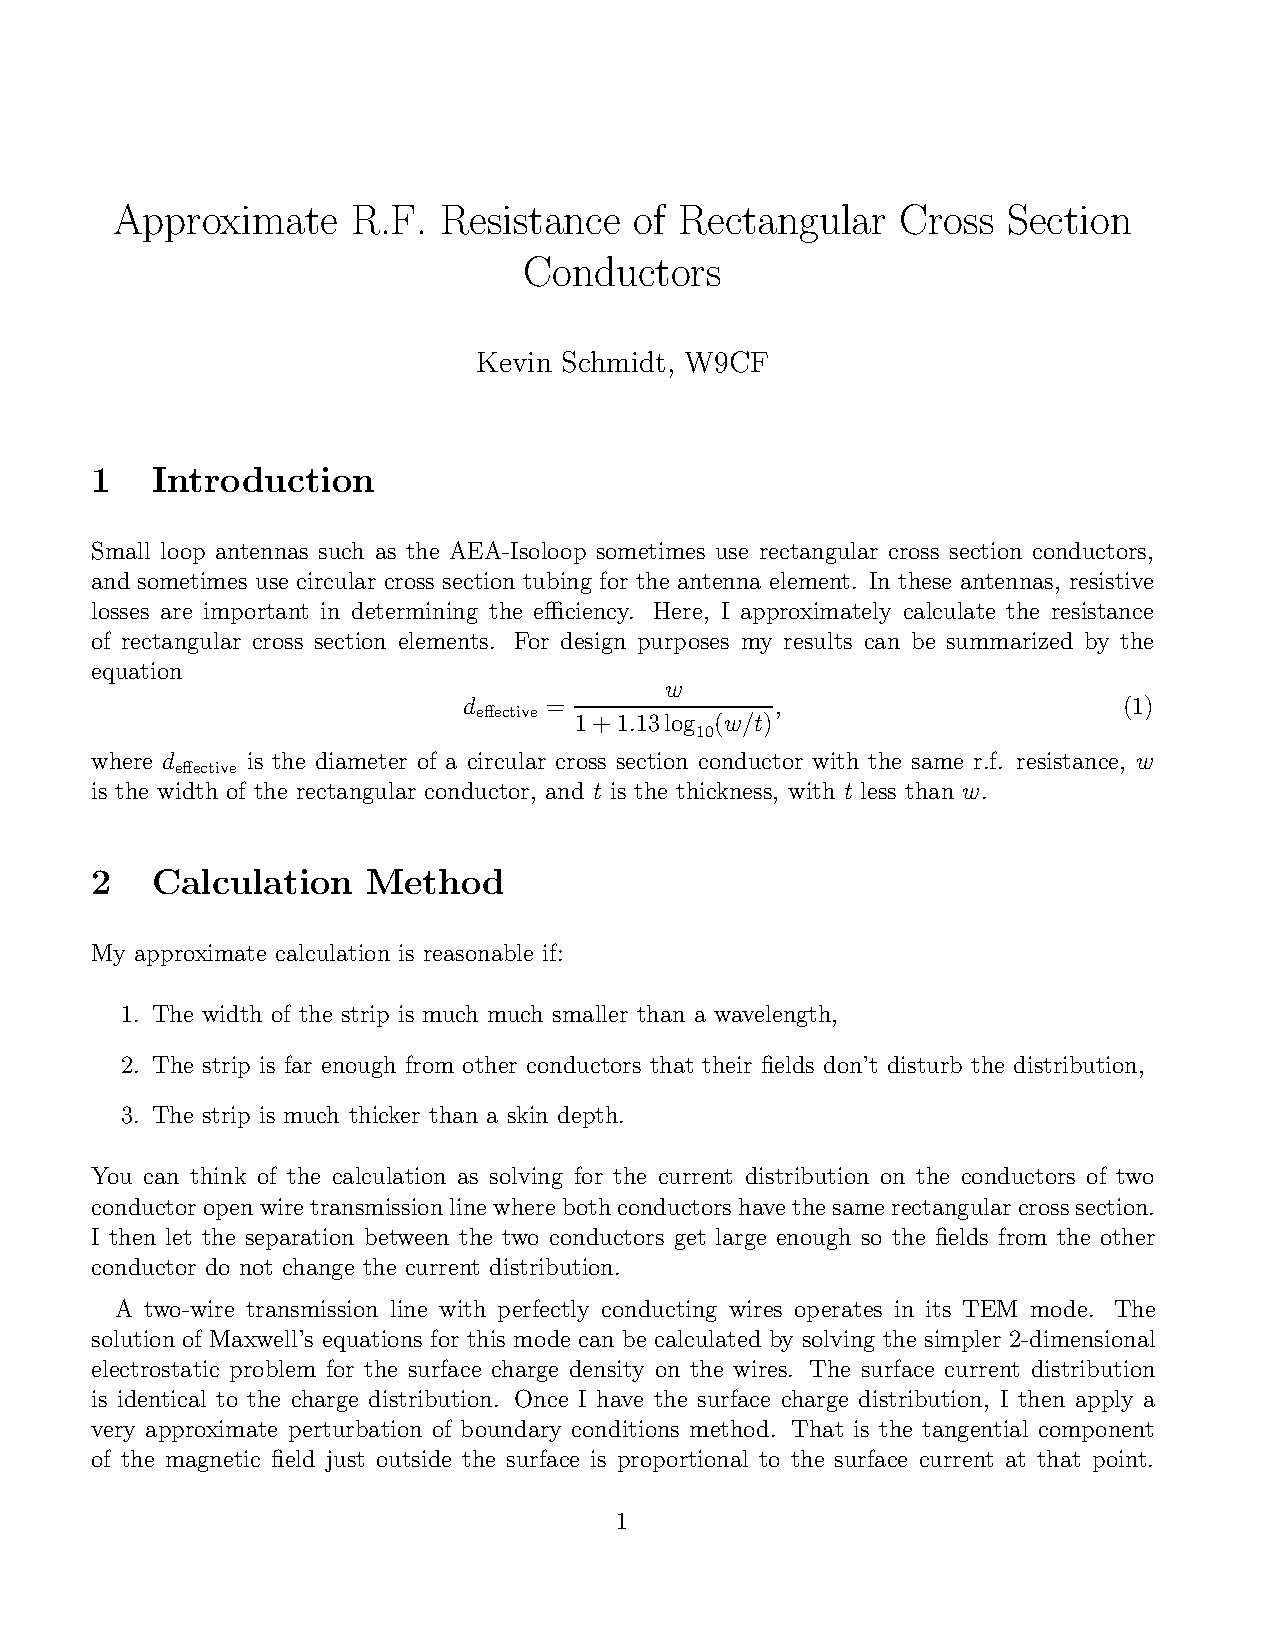
\includegraphics[width=3in]{equiv.fig2}}
\end{figure}%
\lthtmlfigureZ
\hfill\lthtmlcheckvsize\clearpage}

{\newpage\clearpage
\lthtmlfigureA{figure54}%
\begin{figure}

\rotatebox {270}
{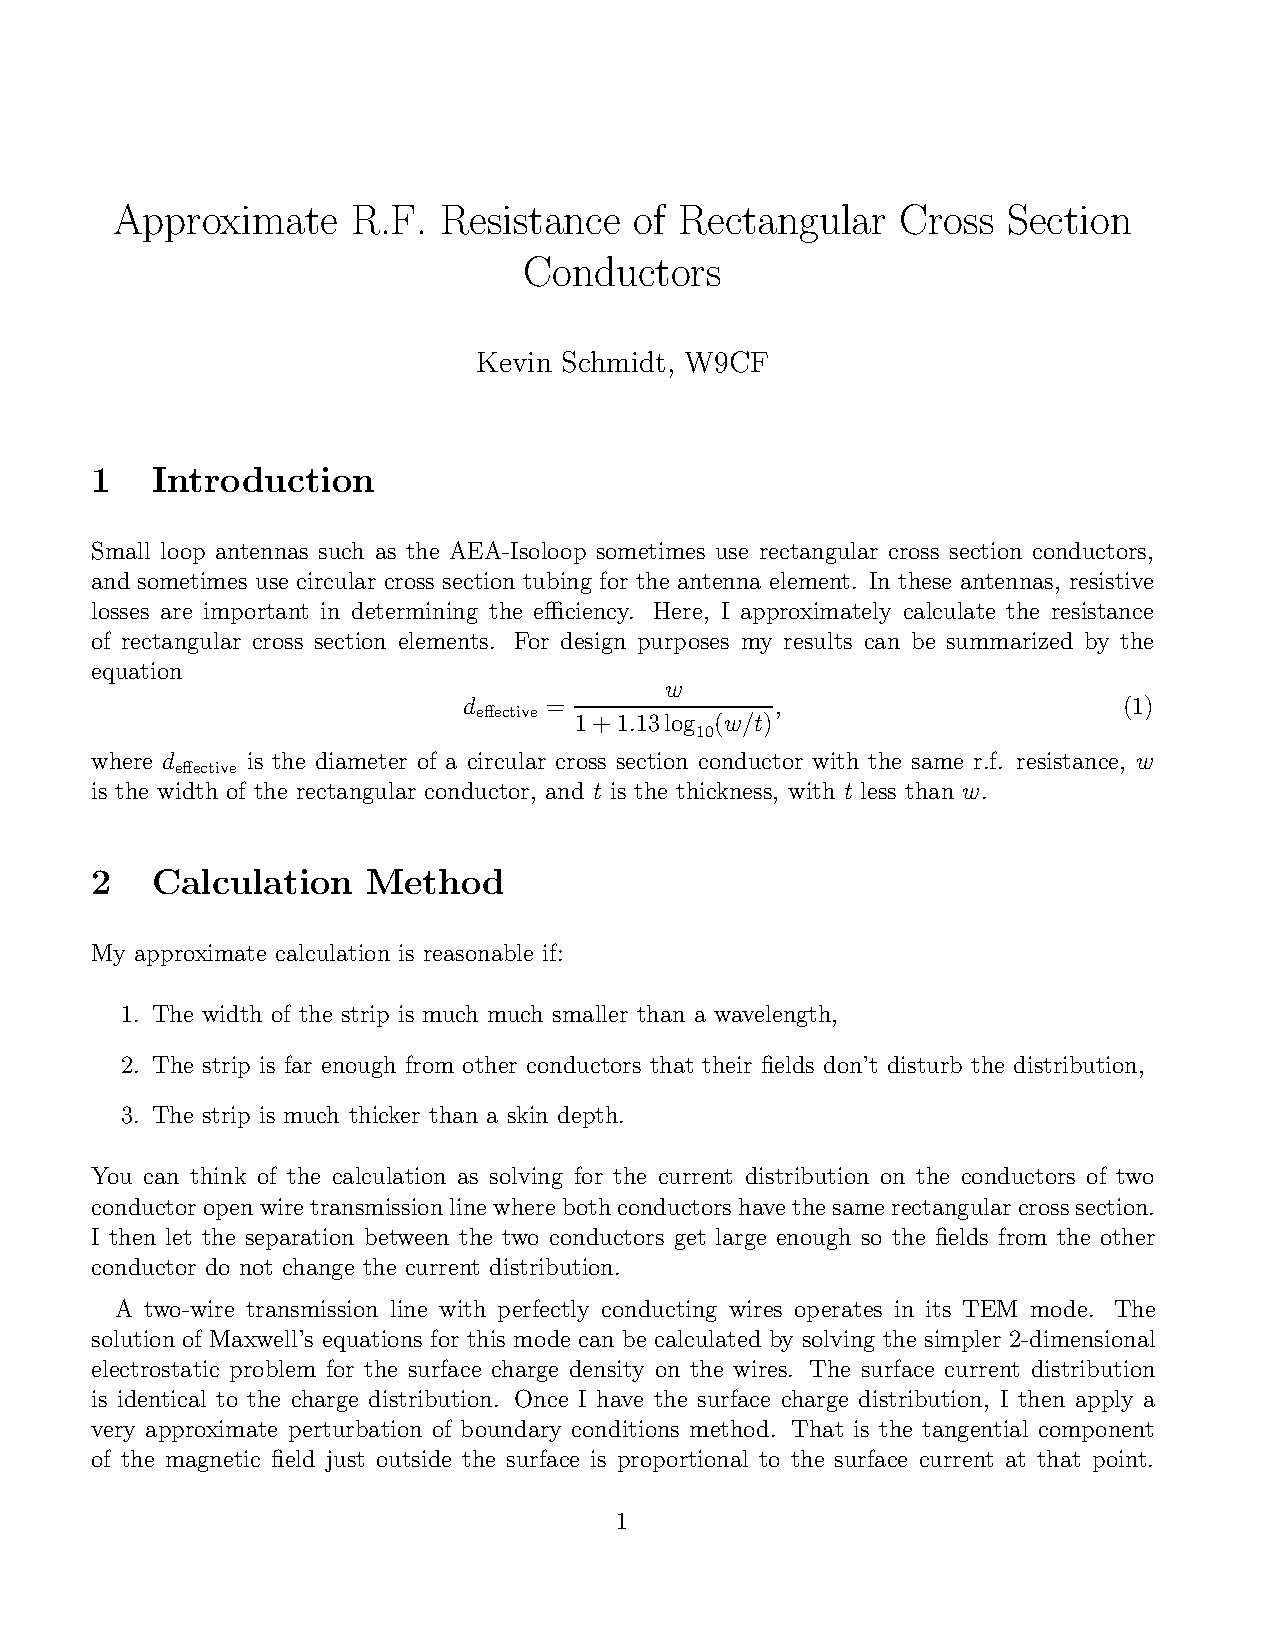
\includegraphics[width=3in]{equiv.fig3}}
\end{figure}%
\lthtmlfigureZ
\hfill\lthtmlcheckvsize\clearpage}

\stepcounter{section}
{\newpage\clearpage
\lthtmlfigureA{figure71}%
\begin{figure}

\rotatebox {270}
{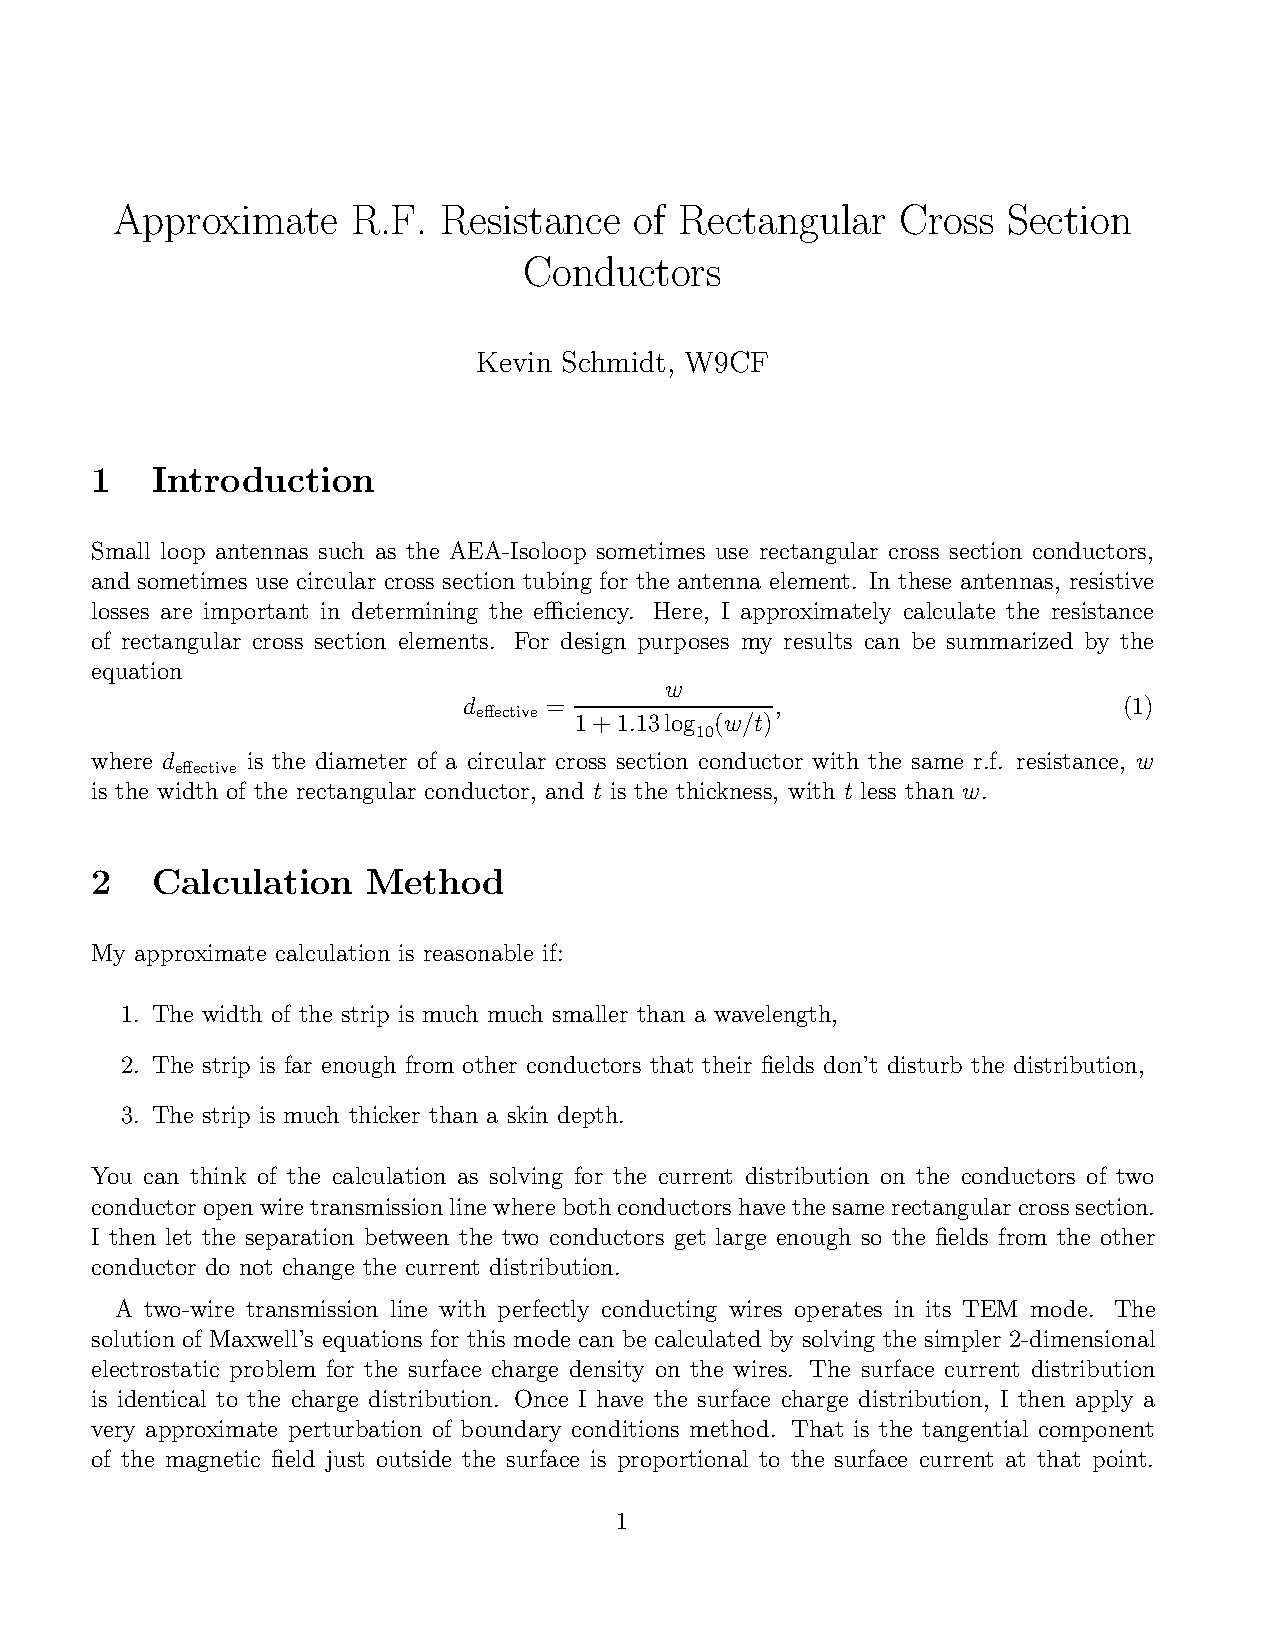
\includegraphics[width=3in]{equiv.fig4}}
\end{figure}%
\lthtmlfigureZ
\hfill\lthtmlcheckvsize\clearpage}

\stepcounter{section}
{\newpage\clearpage
\lthtmlinlinemathA{tex2html_wrap_indisplay437}%
$\displaystyle\alpha$%
\lthtmlinlinemathZ
\hfill\lthtmlcheckvsize\clearpage}

{\newpage\clearpage
\lthtmlinlinemathA{tex2html_wrap_indisplay438}%
$\displaystyle\left [1/h(inches) \sqrt{f(MHz)} \right]$%
\lthtmlinlinemathZ
\hfill\lthtmlcheckvsize\clearpage}

{\newpage\clearpage
\lthtmlinlinemathA{tex2html_wrap_inline440}%
$\alpha$%
\lthtmlinlinemathZ
\hfill\lthtmlcheckvsize\clearpage}

{\newpage\clearpage
\lthtmlinlinemathA{tex2html_wrap_inline443}%
$\alpha$%
\lthtmlinlinemathZ
\hfill\lthtmlcheckvsize\clearpage}

{\newpage\clearpage
\lthtmlinlinemathA{tex2html_wrap_inline456}%
$\pi$%
\lthtmlinlinemathZ
\hfill\lthtmlcheckvsize\clearpage}

{\newpage\clearpage
\lthtmlinlinemathA{tex2html_wrap_inline459}%
$\infty$%
\lthtmlinlinemathZ
\hfill\lthtmlcheckvsize\clearpage}

{\newpage\clearpage
\lthtmlinlinemathA{tex2html_wrap_inline461}%
$\infty$%
\lthtmlinlinemathZ
\hfill\lthtmlcheckvsize\clearpage}

{\newpage\clearpage
\lthtmlinlinemathA{tex2html_wrap_inline463}%
$\infty$%
\lthtmlinlinemathZ
\hfill\lthtmlcheckvsize\clearpage}

{\newpage\clearpage
\lthtmlinlinemathA{tex2html_wrap_indisplay473}%
$\displaystyle{\frac{w}{1+\log_{10}(w/t)}}$%
\lthtmlinlinemathZ
\hfill\lthtmlcheckvsize\clearpage}

\stepcounter{section}

\end{document}
